% 2018 江苏卷第17题：农田大棚温室几何图
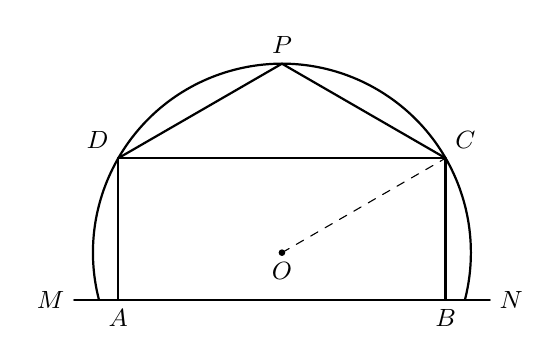
\begin{tikzpicture}[font=\small, line cap=round, line join=round, >=stealth, scale=0.06]
  % 圆心与原点
  \coordinate (O) at (0, 0);
  \coordinate (P) at (0, 40);
  \coordinate (M) at (-44, -10);
  \coordinate (N) at (44, -10);

  % 绘制底边线段 MN
  \draw[thick] (M) -- (N);

  % 绘制圆弧 MPN
  \draw[thick] (-38.73, -10) arc (194.48: -14.48: 40);

  % 矩形 ABCD
  \coordinate (C) at (34.64, 20);
  \coordinate (D) at (-34.64, 20);
  \coordinate (B) at (34.64, -10);
  \coordinate (A) at (-34.64, -10);

  \draw[thick] (A) -- (B) -- (C) -- (D) -- cycle;

  % 三角形 CDP
  \draw[thick] (D) -- (P) -- (C);

  % 连结 OC
  \draw[dashed] (O) -- (C);

  % 标记点与标签
  \fill (O) circle (20pt) node[below] {$O$};
  \node[above] at (P) {$P$};
  \node[above left] at (D) {$D$};
  \node[above right] at (C) {$C$};
  \node[left] at (M) {$M$};
  \node[right] at (N) {$N$};
  \node[below] at (A) {$A$};
  \node[below] at (B) {$B$};
\end{tikzpicture}
